% Copyright (c) 2014,2016 Casper Ti. Vector
% Public domain.

\chapter{利用CNN分辨NLDBD事件和背景事件}
\label{chapter:cnn}

正如上文所述,NLDBD事件是一个及其稀有的事件,其半衰期超过了$1.07\times10^{26}$年,因而对于实验中的本底控制提出了很高的要求。根据第\ref{chapter:background}章所进行的背景模拟数据,PandaXIII实验中200kg级的探测器每年会探测到约78个本底$\gamma$事件落在ROI能量区间中,这个事件率还是远远高于实验的需求,因而需要一些其他的方式来压低本地信号,其中最自然的方法便是利用事件径迹的相关信息来区分背景事件和NLDBD事件。

NLDBD事件会同时释放出两个高能电子,在其径迹的两个末端会有这十分明显的布拉格峰,这是NLDBD事件最为明显的一个特征。而传统的$\gamma$本底事件一般通过一次或多次康普顿散射产生一个或多个次级电子,所以$\gamma$射线的径迹会形成一个或多个单末端布拉格峰的径迹。所以如果我们能够得到探测器探测到事件的详细径迹信息,就可以由此高效的分辨出本底事件和NLDBD事件,从而极大的压低本地。

然而因为PandaXIII读出系统的限制,使用传统的方法重建径迹会变得比较困难,因而我们探究了使用CNN深度神经网络来进行事件鉴别这一方法,得到了较为优异的效果。本章节详细描述了利用CNN进行事件鉴别的动机,CNN模型的选择和搭建,数据处理和训练等细节,希望能够帮助读者建立起对于CNN清晰简单的认识,为高能物理研究甚至是其他领域的研究提供相应的帮助。

\section{传统鉴别方法以及遇到的困难}

如前文所述,NLDBD是一个径迹特征即为明显的事件,该特征能够极大地帮助实验的进行。图\ref{fig:samples}给出了NLDBD和背景事件的对比,可以很明显的看出NLDBD事件径迹在末端拥有两个明显的布拉格峰,而背景$\gamma$事件则只存在一个布拉格峰。如果我们的TPC能够完美的重建出事件的径迹信息,那么鉴别该事件是否是NLDBD事件就会变得及其的简单:我们只要重建出径迹沉积的能量随径迹位置的关系,然后使用简单的cut就可以判断该事件的类型。然而在PandaXIII中重建径迹这个操作是十分困难的,原因如下。

\begin{figure}[hbt]
    \centering
    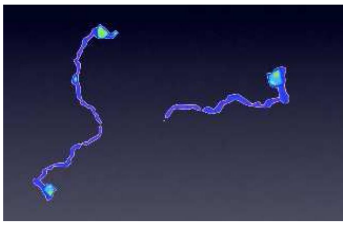
\includegraphics[width=0.5\columnwidth]{pic/fig10.png}
    \caption{一个NLDBD事件(左图)和一个$\gamma$背景事件(右图)径迹投影图。可以很明显的分辨出左侧径迹末端有两个布拉格峰,而右侧只有一个末端有布拉格峰。}
    \label{fig:samples}
\end{figure}

PandaXIII设计使用了41个Microbulk Micromegas读出板来构建读出平面,每个MM(Microbulk Micromegas)板的尺寸为20厘米x20厘米,按照图\ref{fig:mms}所示的形状排列组成,这样的话读出平面能够极大的覆盖漂移区域,从而提升事件的探测效率。

\begin{figure}[hbt]
    \centering
    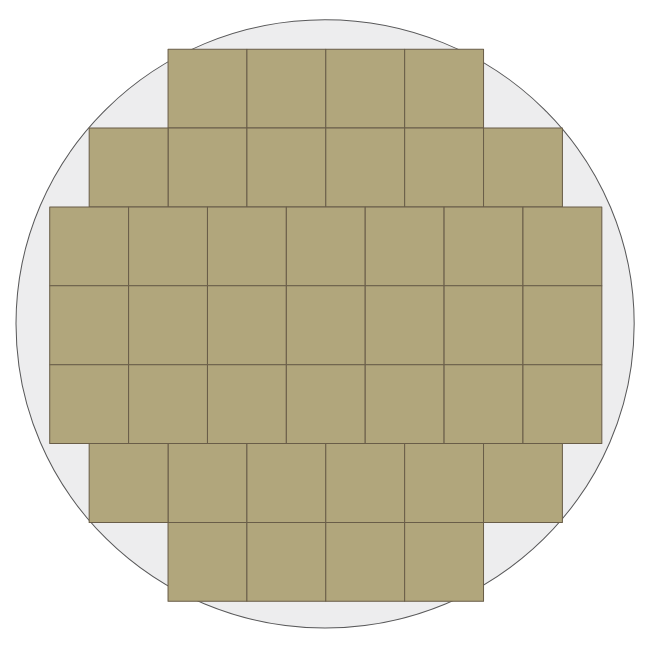
\includegraphics[width=0.4\columnwidth]{pic/fig8.png}
    \caption{41个MM板组合探测器读出平面排放示意图,按照4,6,7,7,7,6,4层叠放置。}
    \label{fig:mms}
\end{figure}

如图\ref{fig:mm_detail}左图所示,每个MM上都密布了许多增益孔(Amplification holes),用于采集漂移到附近的电子。这些增益孔按照合适的排布组成菱形的读出像素,每个像素的对角线尺寸约为3毫米,这边是Micromegas的位置分辨率。如果MM采取像素读出的话,一块MM会拥有约4000个通道(channel),整个TPC则会超过32万,这么多道数对于电子学部分基本是不可以承受的,因而PandaXIII使用了条状读出,而不是像素读出。如图\ref{fig:mm_detail}右图所示,每一组红色像素被连接在一起,在Y方向上形成64个通道,X方向上同样由黄色像素组成64个通道。这样的话一块MM读出板只会形成128个通道,从而大大降低了电子学的复杂程度。

\begin{figure}
    \centering
    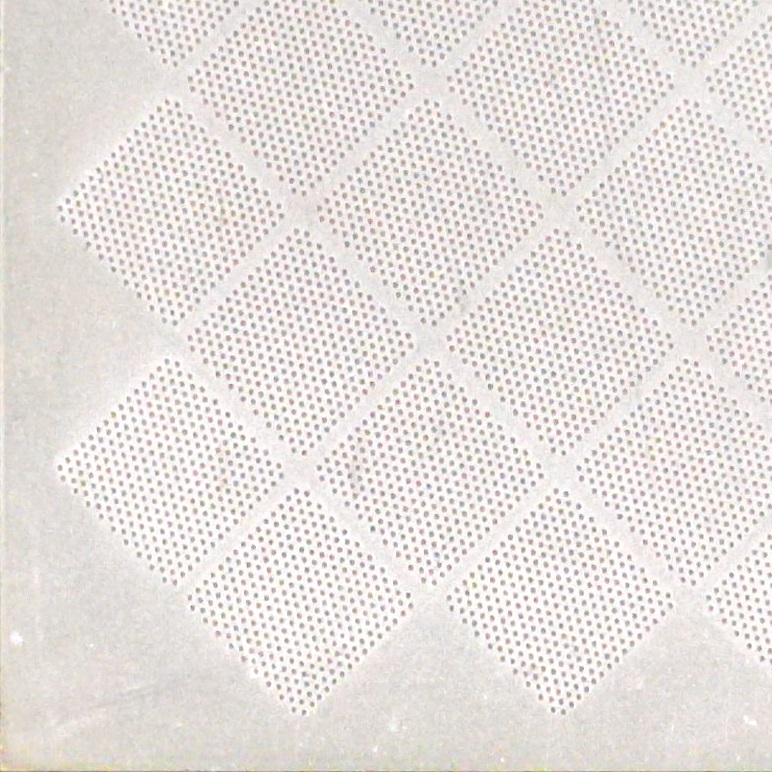
\includegraphics[width=0.4\columnwidth]{pic/MMStrips.jpg}
    \includegraphics[width=0.4\columnwidth]{pic/MMPattern.pdf}
    \caption{左图,MM板局部读出区域的放大示意图,图中的小孔便是增益孔(Amplification Holes),若干孔组成一个菱形读出像素,每个像素的对角线长度约为3毫米。右图:MM板局部读出通道(channel)连接示意图,红色以及黄色菱形(正方形)区域即为中图所示的读出像素,每一条红色虚线或者黄色虚线连接了一组读出像素,形成一个读出通道。\supercite{lin2018design}}
    \label{fig:mm_detail}
\end{figure}

但是采取条状读出也有对应的弊端,即我们无法同时获取到漂移到MM读出板上电子的X和Y的位置,我们只能得到它的X\textbf{或}Y的位置。再加上通过漂移时间计算得到的Z轴相对位置关系后,我们能够轻易的得到一个事件的X-Z-energy投影信息和Y-Z-energy投影信息,而有关X-Y的信息则因为MM结构问题而被彻底抹去了,这就使得重建径迹的3维信息变得极其的困难。

虽然一条比较直的径迹可以紧紧通过X-Z以及Y-Z来组合得到X-Y-Z的径迹,但是电子在TPC中的运动径迹往往不规则,同一时刻往往会有超过一组X和Y读出条被触发,这样同一Z值(同一时刻)的XY信息就无法确定,如图\ref{fig:difficulty_track_2}所示。如果两个真实的hit分别位于($x_1$,$y_1$)和($x_2$,$y_2$),那么因为条状读出的原因,$x_1,x_2,y_1,y_2$所在的通道会同时被触发,那么重建就可能得到错误的能量沉积点。图\ref{fig:difficulty_track}便给出了一个难于重建的
NLDBD事件投影图,该事件在Z在(80,110)毫米处的径迹纠缠在了一起,所以基本上不可能完成重建。

\begin{figure}
    \centering
    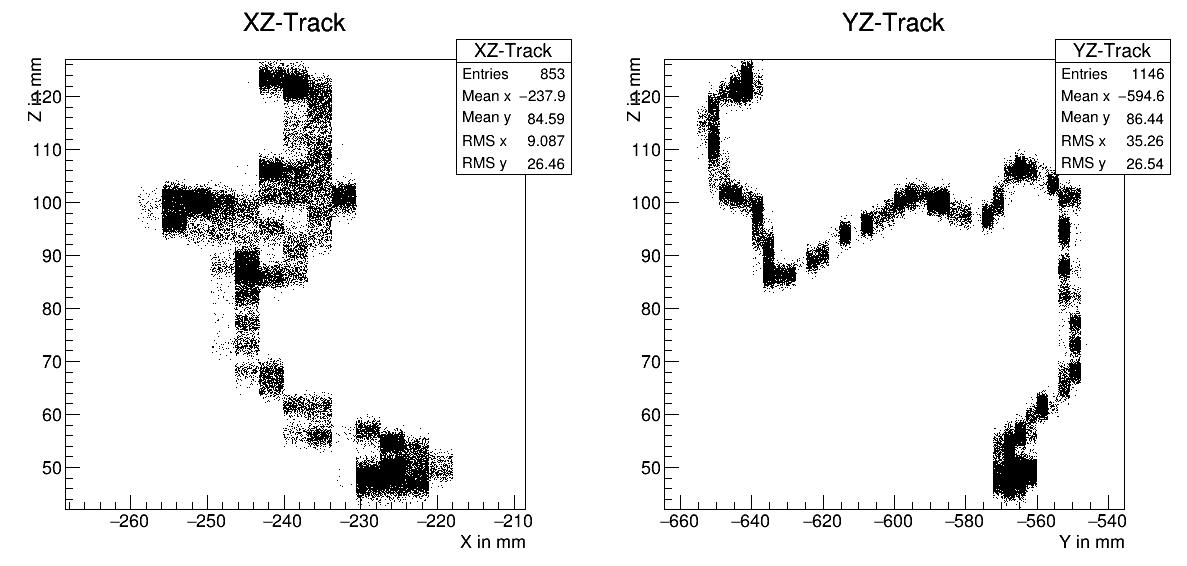
\includegraphics[width=0.7\columnwidth]{pic/difficulty_track.png}
    \caption{一个难于重建的事件的XZ投影和YZ投影,区块深浅表示沉积能量的大小,Z在(80,110)毫米内的径迹因为X方向上的多种可能而变得无法重建。}
    \label{fig:difficulty_track}
\end{figure}

\begin{figure}
    \centering
    \includegraphics[width=0.4\columnwidth]{pic/app01_strip_readout.pdf}
    \caption{条状读出易混淆的示意图。真实的能量沉积位置如图中绿色点所示($x_1$,$y_1$)和($x_2$,$y_2$),但是因为$x_1,x_2,y_1,y_2$所在的通道同时被触发,因而可能得到红色表示的错误重建结果。}
    \label{fig:difficulty_track_2}
\end{figure}

MM条状读出同时还带来了另外一个困难,因为一个电子要么落在X读出条所在的像素中,要么落在Y读出条所在的像素中,因而径迹相同位置在重建后的两个投影处的能量并不相等。所以根据能量的大小做X-Y的匹配也困难重重。作者个人认为在使用MM条状读出的前提下,能够良好的重建出径迹基本是不可能的,因而需要探寻新型的事件鉴别的方式方法。于是我们便试图将近年来在计算机领域大放异彩的深度神经网络引入我们的粒子鉴别,以期望它能够解决这个难题。

\section{CNN介绍以及使用动机}

\subsection{使用动机}
正如上文所说的,使用MM作为读出时很难通过重建出3维径迹后利用物理图像直接分类,但是如果将形如图\ref{fig:samples}的图片交于人眼来识别,那么相信绝大部分的人都可以轻而易举的分辨出NLDBD事件和背景$\gamma$事件。同时在这个分辨过程中我们并没有试图将两个偷影重建成3维的信息,而是直接通过分析比较两个投影并找到径迹的末端。这种行为操作相对来说难于量化,虽然可能可以通过精细的CUT达成,但是在这些操作的过程中可能需要人工的丢掉大量的数据以降低CUT的复杂度,这都不是我们所希望的。

近些年来随着机器学习技术的快速发展,我们发现似乎CNN真的能够进行一些类似于人类智能的处理,例如Google公司所开发的围棋AI,AlphaGo\supercite{gibney2016google},更是击败了诸多现役棋手,本文会在下一小节详细介绍有关机器学习和CNN的知识。鉴于CNN如此“智能“的表现,我们希望它能够完成类似自然人所做到的事情,即通过观察径迹的两个方向上的投影而做出准确的判断。CNN能够直接将图片作为输入,这样它能够最大限度的利用重建后的信息。同时我们可以通过模拟给CNN提供无比大量的信号样本和背景样本,其他CNN应用场景中最为困难的样本采集和标定对于模拟来说根本不是问题。可以看出CNN非常适合我们的实验需求,而事实上它也较为完美的达到了我们的目标,有关测试的结果见章节\ref{section:cnn_result}。

\subsection{神经网络介绍}

关于神经网络的介绍最早应该从机器学习开始。人们一直在探寻人类自身智慧的来源,从一开始的哲学方面的探讨,再到近代从生物学医学的方向出发,智能一直是科学界中最令人着迷的一个方向。在1949年加拿大心理学家唐纳德·赫布提出了赫布理论\supercite{hebbian},为生物神经网络的学习做出了理论的支撑。1952年IBM的Arthur Samuel开发了一个国际跳棋程序,他发现他构造的这个程序能够随着局数的增多而下得越来越好,因而他给出了机器学习最初的定义,即”不需要显式编程就可以赋予机器某项能力的研究领域“。随后的几十年,机器学习领域一直在慢慢的发展,也分化除了若干个方向,包括1986年由J. R. Quinlan提出的决策树,1995年Vapnik和Cortes提出的支持向量机(Support Vector Machine,SVM)等\supercite{mlhistory}。直到2008年后,英伟达公司所提出的统一计算构架(Compute Unified Device Architecture,CUDA)\supercite{CUDA}的出现,人们利用计算机能够得到的计算能力极大地增强,机器学习中沉寂了许多年的神经网络方向才得以快速的发展,重新回到了大众的视线。

无论是递归神经网络(Recurrent Neural Network, RNN),卷积神经网络 
(Convolutional Neural Network,CNN),抑或是对抗神经网络
(Generative Adversarial Network,GAN),他们都离不开神经网络(Neural Network),神经网络最基本的组织单元便被称为神经元(Neural)。每一个神经元都拥有着若干个输入,并通过一定的算法将这些输入和自身存储的参数一起进行处理,给出一个或多个输出。简单而言,对于一组输入$(x_1,x_2,...,x_n)$,单输出的神经元为:
$$ y= f(x_1,x_2,...x_n,a_1,a_2,...,a_m)$$
其中$(a_1,a_2,...,a_n)$是神经元自身的参数,f为某一种非线性函数。当然实际上我们使用的神经元的结构相对简单,一个显著的全连接神经网络中的神经元如下所示:
\begin{equation}
     y=g(\omega_1 x_1+\omega_2 x_2 + ... + \omega_n x_n+ \omega_0))
     \label{eq:neural}
\end{equation}
其中$(\omega_1,\omega_2,...,\omega_n)$被称作权重,$\omega_0$为偏置(Bias),$g(z)$则被成为激活函数(Activation Function),它的主要作用是提供一个非线性的部分。一个典型的被称作sigmod的激活函数表达形式为:
$$g(z)=\frac{1}{1+e^{-z}}$$
显然,一个神经元的输出可以当做另外一个神经元的输入,许多神经元共同组成一个网络,像自然中的神经细胞一样相互影响,共同对输入量做出反应,这就是一个神经网络。然而为了简化模型,我们通常会对网络进行分层研究。

当若干个相似的神经元共同对一组输入做出反应时,我们可以将其称之为一层网络,即$\bar Y = F( \bar X, \omega_1,...,\omega_n)$
其中输入便是一个张量(tensor)$\bar X$,输出则是另外一个张量$\bar Y$。许多不同类型的层相互层叠,每一层的输出作为下一层的输入,最终形成一个
\begin{equation}
    \bar Y_0 = \mathcal{F}(\bar X_0, \mathcal{W})
\end{equation}的非线性系统。而神经网络的训练便是寻找最能够拟合已知输入输出的参数们$\mathcal{W}$。图\ref{fig:simple_nn}展示了一个简单的全连接神经网络示意图,该网络接受一个维度(shape)为(3)的张量作为输入,并输出一个维度为(1)的张量(标量)。

\begin{figure}
    \centering
    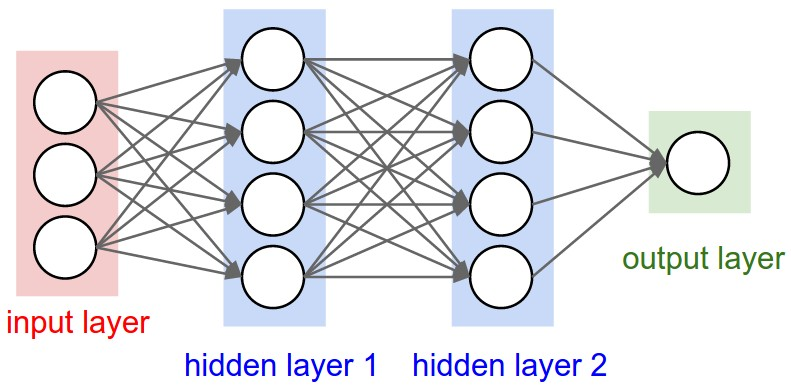
\includegraphics[width=0.7\columnwidth]{pic/simple_nn.jpeg}
    \caption{一个简易的全连接神经网络,包含一个输入层,两个隐含层以及一个输出层。}
    \label{fig:simple_nn}
\end{figure}

一个神经网络中所有神经元的参数便被成为这个网络的权重(Weight),而神经网络中的层的类型和层的属性(神经元数目,组合方式)则被称作模型(Model)。如果我们要试图使用神经网络来解决问题,我们就需要按照下面的步骤进行:
\begin{enumerate}
    \item 确定网络的输入和输出,即明确问题的输入张量和输出张量。
    \item 根据输入张量输出张量以及问题的特性构造合适的模型。
    \item 准备足够的包括输入和输出的样本数据。
    \item 使用合适的算法训练模型,得出最符合样本的权重数据。
    \item 使用该模型和训练得到的权重去预测未知的输入。
\end{enumerate}
在PandaXIII中,我们的问题是使用神经网络来鉴别一个事件是NLDBD事件或者是背景事件,这是一个非常明确的二分类问题。即我们的输入是事件的信息,输出是事件的类型。我们通过将会选择几个模型,使用MC生成的数据加以训练和测试,从中挑选出最为合适的网络并最终用于真实的实验数据中。

\subsection{CNN以及其他类型神经网络介绍}

卷积神经网络(Convolutional Neural Network)现在神经网络相关领域中机器重要的一部分,它广泛应用在图像识别的相关方向。相对于普通的全连接网络,CNN的核心便是模型中拥有卷积层。一个简单的二维卷积操作如公式\ref{eq:con}所示。卷积神经网络处理的一般是图片,因而输入数据一般是一个二维的张量,它与一个被称作卷积核的参数矩阵做卷积操作,并将结果输出,这就形成了卷积层中的一个神经元。图\ref{fig:con}给出了另外一个正在进行的卷积操作示意图。
\renewcommand\arraystretch{1.0}
\begin{equation}
    Input(\left[ \begin{array}{ccccc}
        1&1&1&0&0\\
        0&1&1&1&0\\
        0&0&1&1&1\\
        0&0&1&1&0\\
        0&1&1&0&0
    \end{array} \right])
    \otimes Convolutional Core(\left[ \begin{array}{ccc}
        1&0&1\\
        0&1&0\\
        1&0&1
    \end{array} \right]) = Output(\left[ \begin{array}{ccc}
        4 &3 &4\\
        2 &4&3\\
        2&3&4
    \end{array} \right])
    \label{eq:con}
\end{equation}

\begin{figure}
    \centering
    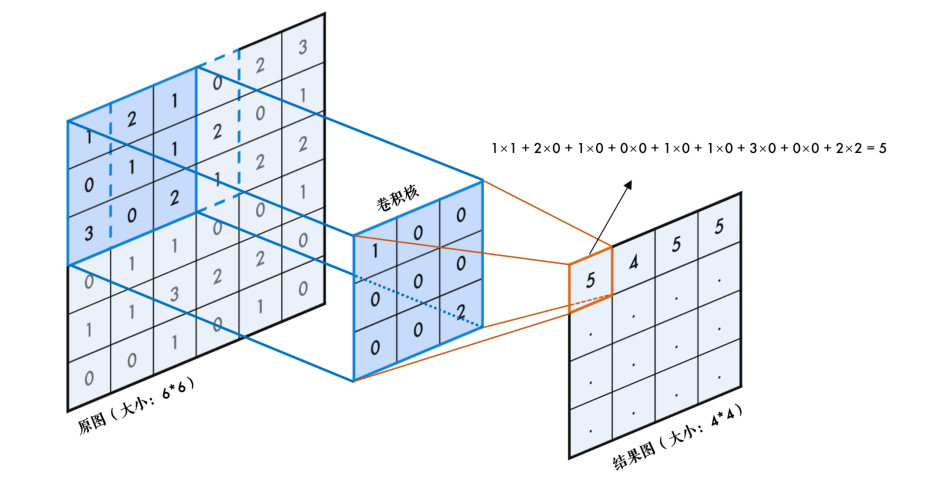
\includegraphics[width=0.7\columnwidth]{pic/con.jpg}
    \caption{一个正在进行的卷积操作示意图\supercite{con}。}
    \label{fig:con}
\end{figure}

一层卷积层便是由N个卷积神经元所组成,每个卷积神经元都有一个$M \times M$的卷积核。因而对于一个输入维度(X,X)的张量,卷积层使用了$N\times M\times M$个参数对输入数据进行处理,输出张量的维度为(N,X-M+1,X-M+1)。而如果试图使用全连接层网络寻找图片的N个特征,那么全连接层的参数数目将会是$N\times X\times X$,远远大于卷积层的参数数目。所以说相对于全连接层,卷积层认为图片的局部特征是有一定的关联性和通用性的,因而可以较小参数的卷积核来表征和卷积操作来表示和提出该特征,从而在大大降低参数数目和计算复杂度的情况下依然拥有着良好的效果。

除了卷积神经网络之外,我们通常还会提到深度神经网络(Deep Neural Network),它的核心便是网络层数多切复杂,网络比较”深“。一般来说,相对于机器学习中的神经网络,拥有两个及以上隐藏层的网络便可以被称作深度神经网络。但是在神经网络中,越是复杂的网络越需要细致的设计和优化调整来达到更为优异的效果,因此在处理具体问题中,相对出从零开始构造一个深度神经网络,尝试和修改既有的深度神经网络更为可行。

递归神经网络(Recurrent Neural Network, RNN)则更适用于处理自然语言识别等相关领域。相对于普通的全连接网络,递归神经网络考虑到了每一层内神经元之间的相互作用,即每次训练中递归层的结果会影响到下一次训练的过程中。因而递归神经网络可以提取数据序列中的相对关系,对于自然语言处理,时间序列数据的处理更为合适。

对抗生成神经网络(Generative Adversarial Network)则是一种特殊的训练网络方式,它使用数据同时训练两个神经网络,一个用于从噪声中生成数据,另一个则鉴别生成器生成的数据,两个网络相互之间不停地对抗,即生成网络试图生成鉴别网络无法区分的数据,而鉴别网络则在努力的识别出由生成网络生成的数据。因而GAN可以从既有的样本中提取信息,并生成类似的数据。

\section{数据准备}
\label{section:data_prepare}

\subsection{输入数据和输出数据的格式}
如上文有关神经网络介绍中的所述,我们使用CNN进行事件鉴别首先要明确问题的输入和输出。对于PandaXIII实验而言,我们希望CNN能够尽量多的利用既有的数据,并由此给出事件的类型。从探测器读出的结构以及先前进行的模拟工作来看,我们的探测器可以很方便的重建出一个事件在X-Z-energy以及Y-Z-energy这两个方面上的投影,因而我们CNN的输入便是这两组数据。根据先前所描述的动机以及CNN网络的特性,每个事件两个投影应该被合并转换成一张图片作为CNN的输入,而输出则是一个在(0,1)范围内的小数,代表着该事件更类似于一个背景事件(0)或者是一个信号事件(1)。

PandaXIII实验设计中读出电子学部分将会以5MHz的频率采样512个时间点,即采样$102\mu s$的数据,而电子在气体中的漂移速度为$1.87 mm/ \mu s$,那么一个时间在Z方向上的最长长度约为190 mm。 MM读出在X及Y方向上的像素尺度为3mm,考虑到时间在探测器中的径迹应该是各项同性的,所以我们希望我们得到的数据中X,Y,Z的地位也是一致的,因而我们转换完成的图片中每个像素的值都代表着$3\times 3mm^3$区域内沉积的能量,图片尺寸最大不超过63个像素。因而为了方便,我们最终决定使用$60\times60$像素的图片作为CNN网络的输入。

我们重建每个事件都会得到两个投影,而CNN一般只接受一张图片作为输入,因而我们需要将两个投影所转换出的两张图片合并成一张。因为每个投影所转换出的图片都是一个灰度图片,同时CNN神经网络可以接收彩色图片作为输入,所以我们将X-Z投影转换出的图片数据放置在红色通道,Y-Z投影放置在绿色通道,这样就可以将两张灰度图片转换为一张彩色图片,从而交于CNN进行训练和识别了。同样的方法也被NEXT-100实验所采用\supercite{renner2017background}。

\subsection{NLDBD事件及背景事件的模拟数据生成}

在明确CNN网络的输入和输出之后,我们就需要去准备数据以供CNN训练和测试所用。虽然NLDBD事件至今没有被探测到,但是依然可以根据相关的理论来模拟出它的具体信息。在PandaXIII实验中我们使用了DECAY0软件包\supercite{ponkratenko2000event}来生成NLDBD事件发生后释放出的两个电子的动量信息,并将其随机放置在漂移时的气体内,作为BambooMC模拟框架的输入。和章节\ref{chapter:background}中的模拟工作相类似,模拟可以得到NLDBD事件在探测器中hit的相关信息,其沉积能量能谱如图\ref{fig:nldbd_energy}左所示。

\begin{figure}
    \centering
    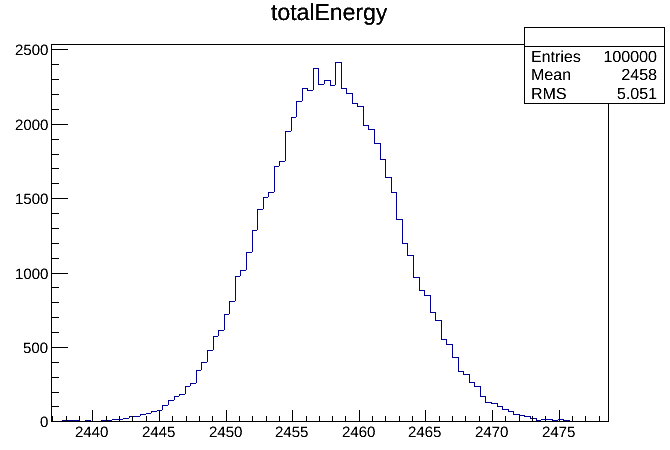
\includegraphics[width=0.3\columnwidth]{pic/nldbd_raw_spectrum.png}
    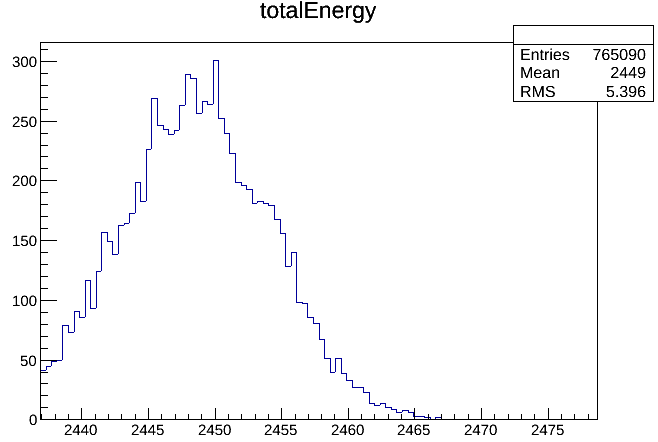
\includegraphics[width=0.3\columnwidth]{pic/2447_raw_spectrum.png}
    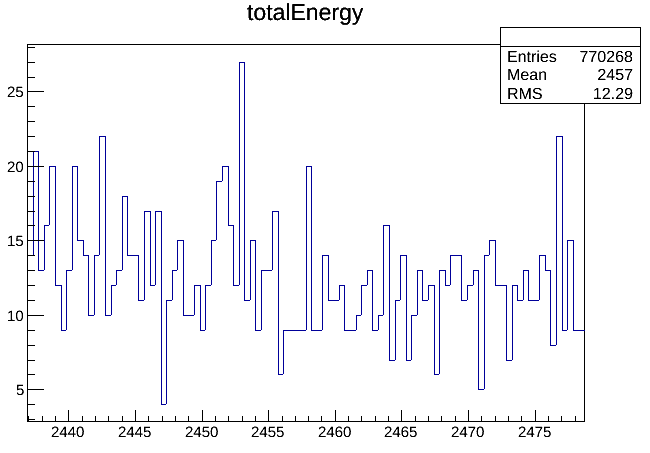
\includegraphics[width=0.3\columnwidth]{pic/2614_raw_spectrum.png}
    \caption{CNN准备数据中BambooMC模拟出的事件能谱图。左:NLDBD事件,中:2447keV$\gamma$本底事件,右:2614keV$\gamma$本底事件}
    \label{fig:nldbd_energy}
\end{figure}

对于背景事件而言,因为在CNN训练中需要准备大量的背景数据,因而像背景模拟一样进行U和Th的全链模拟代价过于高昂。同时因为探测器的背景来源主要是来自于$^{214}$Bi的2447.8keV和$^{208}$Tl的2615.keV$\gamma$射线,所以我们直接将这两个能量的$\gamma$粒子放置在探测器的铜罐中作为起始事件进行模拟,其能谱如图\ref{fig:nldbd_energy}中图和右图所示。在这里我们做了两个近似,即使用两个$\gamma$事件代替真实的U,Th本底事件,以及使用铜罐作为事件的起始位置。第一个近似可以进行的原因是我们期待CNN神经网络是通过识别图片特征来做本底背景的分离,即CNN不关心事件的总能量。事实上我们在将事件投影转换为图片信息的过程中进行了归一化操作,CNN不会也不能得到事件的总能量信息。第二个近似可行的原因是$\gamma$射线穿透能力相当强,其被探测器探测到的位置于其起始位置关系不大,同时因为我们在转换图片时hit的绝对位置信息也被丢弃了,所以我们认为从铜罐中生成本底信号对结果的影响不大。这两点近似我们在测试训练结果中都进行了验证,参见章节\ref{section:cnn_result}。

\subsection{模拟数据转换为图片}

如图\ref{fig:process}所示,在通过BambooMC蒙特卡洛模拟得到背景和信号的hit信息后,依然需要像探测器背景模拟中一样考虑探测器响应,MM的结构以及电子学读出设计对于事件的影响,依此将蒙特卡洛得到的原始hit信息转换为电子学每个通道的波形信息。在得到每个事件的波形信息后,通过读出系统道数和位置的关系再重建出事件的X-Z-energy以及Y-Z-energy投影,并最终将其合并转换为图片供CNN神经网络所使用。各个转换步骤的细节如下:

\begin{figure}
    \centering
    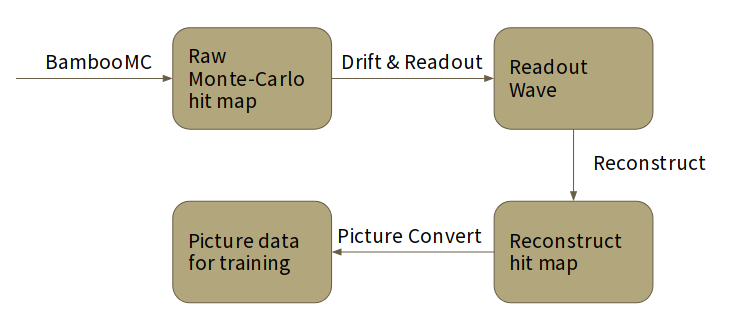
\includegraphics[width=0.6\columnwidth]{pic/process.png}
    \caption{模拟数据转换为CNN所需要的图片过程示意图。}
    \label{fig:process}
\end{figure}

\subsubsection{探测器响应}
    在CNN数据准备中对于探测器相应的处理和背景模拟中的处理完全一致。

\subsubsection{读出结构}
    探测器两端各有一个读出平面,分辨由41个MM读出板组件构成,如图\ref{fig:mms}所示。每个MM读出板的尺寸是200毫米x200毫米,分别拥有64个X读出道以及Y读出道,因而探测器一端拥有5248个读出道。在处理过程中我们需要完整的构建读出平面的结构以及MM读出板的细节结构,从而能够精确得到读出平面(x,y)位置处所述的通道信息,并由此将考虑到探测器响应后电离电子漂移到读出板的位置时间信息(vector<x,y,t>)转换为波形信息(map<channel\_id, vector<count>>)。

    对于MM的处理中有一点需要注意,虽然MM的有效像素并没有完整的覆盖$20\times20cm^3$
    的面积,但是因为电压是直接加在读出像素上的,电子会在电场的作用线漂移到距离靠近的读出像素,并不会因为所在位置处不是读出像素而没有被MM收集到。关于读出板的具体细节以及实现请参考PandaXIII中期报告\supercite{cdr}。

\subsubsection{电子学触发}
    类似于前文背景模拟中关于电子学触发的处理方法,我们在CNN数据准备中一样的使用了5MHz的采样率和512个采样点,触发能量为$Q_{\beta\beta}/2$。事实上电子学触发中关于触发能量的选择正是基于NLDBD事件的模拟数据,即我们希望通过合理的选择触发能量使得在NLDBD事件的效率最高。图\ref{fig:trigger_select}中展示了电子学触发能量对于NLDBD事件探测效率以及能量分辨率的影响,可以看出当触发能量在$Q_{\beta\beta}/2$附近时,能够通过触发的NLDBD事件效率最高。

    \begin{figure}
        \centering
        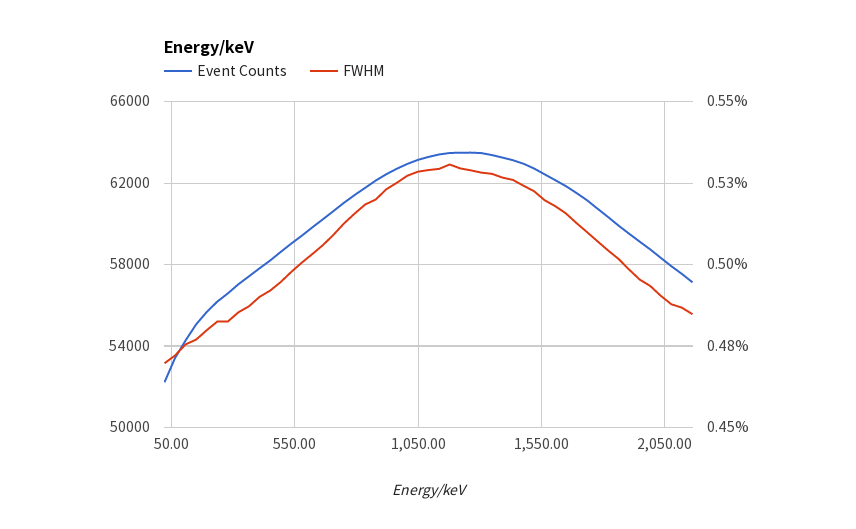
\includegraphics[width=0.8\columnwidth]{pic/trigger_select.png}
        \caption{电子学触发能量对于NLDBD事件探测效率(蓝线,左轴)以及相对能量分辨率(红线,右轴)的影响。其中蓝线表示完成触发的NLDBD事件数目与触发能量的关系,红线表示了探测得到的NLDBD事件能量分辨率随触发能量的变化关系。总模拟事件的数目为100000。}
        \label{fig:trigger_select}
    \end{figure}

\subsubsection{重建}

    在考虑到探测器响应,读出结构以及电子学触发的相关影响后,原初BambooMC模拟得到的hit信息已经被转换为了各个读出通道的波形信息,即在建成探测器后真实采集到的数据信息也是这个格式。接下来我们就需要将波形信息重建回详细的事件径迹信息。

    对于一个事件中每个通道而言,我们可以得到该通道具体所在的位置X或者Y,波形中的时间信息可以通过电子的漂移速度转换为Z左边,对应时间点的强度信息(电子数目)则可以依据探测器的$W$计算出对应的沉积能量。总结而言我们可以十分简易的将波形信息转换为两个二维直方图(Histogram),Z方向上有512个bins,间隔为0.374mm,X或者Y方向上最多有448个bins,间隔为3mm,直方图的计数信息在代表着在对应bins处所沉积的能量大小。

\subsubsection{图片转换}
    重建后得到的两个直方图即为事件在X-Z-energy和Y-Z-energy上的两个投影。我们分别计算出两个投影以能量为权重的位置重心,并以该位置为中心,按照3mm的尺寸重新划分(rebin)直方图,并丢弃超过60x60范围外的数据信息,此时两个投影被转变为两个60x60尺寸的直方图。对于每个直方图,我们都可以将其映射为一张60x60pixels的灰度图片,每个像素灰度的大小即代表着沉积能量的大小,能量最大的点所对应的灰度值为255。在进行图片转换后,事件总能量的信息,以及hit的绝对位置信息都被丢弃掉了,因而我们在模拟背景数据中所做的两个近似是合理的。

    \begin{figure}
        \centering
        \begin{subfigure}[t]{0.22\textwidth}
          \centering
          \includegraphics[width=\textwidth]{pic/03_signal_3d_track.pdf}
          \caption{}
        \end{subfigure}
        \begin{subfigure}[t]{0.44\textwidth}
          \centering
          \includegraphics[width=\textwidth]{pic/03_signal_track.pdf}
          \caption{}
        \end{subfigure}
        \begin{subfigure}[t]{0.16\textwidth}
          \centering
          \setlength{\fboxsep}{0pt}
          \fbox{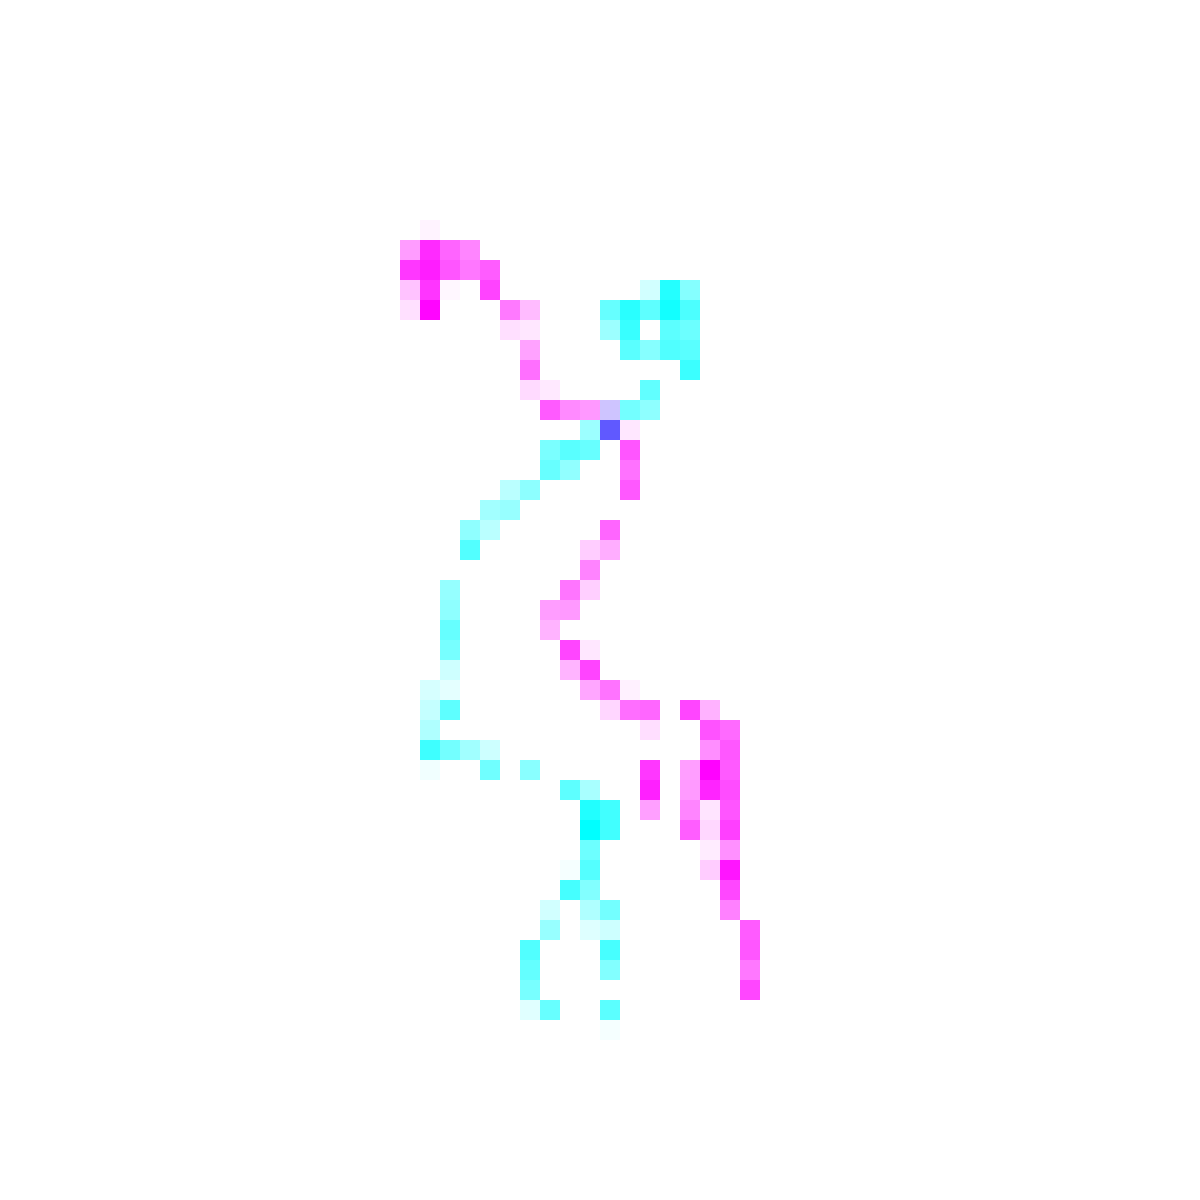
\includegraphics[width=\textwidth]{pic/03_signal_final.png}}
          \caption{}
        \end{subfigure}
        
        \begin{subfigure}[t]{0.22\textwidth}
          \centering
          \includegraphics[width=\textwidth]{pic/03_background_3d_track.pdf}
          \caption{}
        \end{subfigure}
        \begin{subfigure}[t]{0.44\textwidth}
          \centering
          \includegraphics[width=\textwidth]{pic/03_background_track.pdf}
          \caption{}
        \end{subfigure}
        \begin{subfigure}[t]{0.16\textwidth}
          \centering
          \setlength{\fboxsep}{0pt}
          \fbox{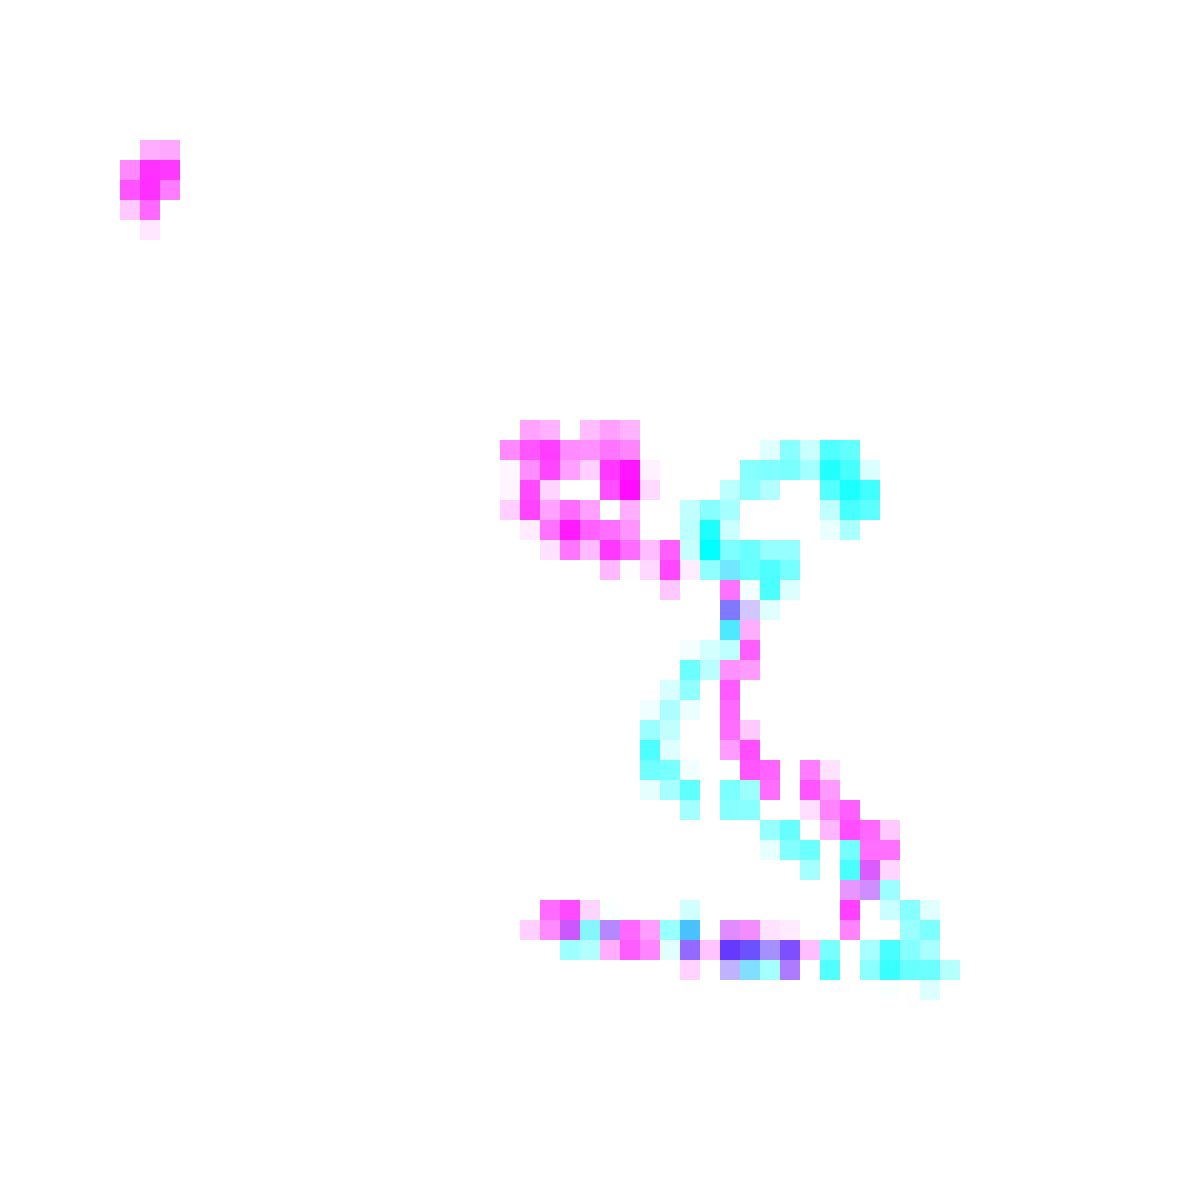
\includegraphics[width=\textwidth]{pic/03_background_final.png}}
          \caption{}
        \end{subfigure}
        
        \caption{NLDBD事件以及背景事件转换示意图。上部分:\xeots NLDBD事件,下部分:2447keV $\gamma$本底事件。(a)和(d):BambooMC模拟得到的3维hit信息。(b)和(e):重建后得到的X-Z-energy 以及 Y-Z-energy投影。(c)和(f):转换完成后的图片示意图,该图片并非CNN训练中所使用的图片,而是为了方便读者观看图片的颜色被后期处理过,其中青色代表着红色通道,粉红色代表着绿色通道。}
        \label{fig:image_mapping}
        \end{figure}

        
\subsubsection{数据转换总结}
图\ref{fig:image_mapping}举例示意了NLDBD事件及$\gamma$本底事件的原始hit信息,重建后的投影信息以及用于CNN训练的图片示意图。我们一共模拟了1百万次NLDBD信号事件以及各$2\times10^9$次
2447keV和2614keV的$\gamma$背景事件,经过上述各个转化过程后所生成的数据规模如表\ref{tab:convert}所示。

我们期望使用CNN来进行一个二分类过程,所以信号和本底的数目应该保持对等,即各占50\%。由于我们的背景是有两部分组成的,虽然根据之前的分析两种背景对于CNN而言应该是没有区别的,但是这里我们还是混合了他们共同作为本底信号,混杂的比例是3.75:1,即无氧铜中U和Th丰都数目比。但需要注意的是,本文并没有研究该比例对实验结果的影响,这一点需要后续的继续研究。我们一共准备了$1.12\times10^6$组信号和背景数据图片,其中80\%被用于神经网络的训练过程中的训练部分(Training dataset),10\%被用于神经网络训练过程中的验证部分(Validation dataset),最后的10\%用于后续的各种测试和检验(Check dataset)。
        
\renewcommand\arraystretch{1.4}
\begin{table*}
    \centering
    \begin{tabular*}{\textwidth}{@{\extracolsep{\fill}}ccccc}
        \hline
        \hline							
        	&	NLDBD	&	2447keV$\gamma$射线	&	2614keV$\gamma$射线	&	合计	\\
        \hline
        MC模拟事件数目	&	$1\times10^6$	&	$2\times10^9$	&	$2\times10^9$	&		\\
        总能量落入ROI事件数目	&	717163	&	3840611	&	1471989	&		\\
        漂移以及触发后事件数目	&	562959	&	1151395	&	485357	&		\\
        触发效率	&	78.50\%	&	30.00\%	&	33.00\%	&		\\
        总体探测效率	&	56.20\%	&	$5.76\times10^{-4}$	&	$2.43\times10^{-4}$	&		\\
        CNN图片数目	&	562959	&	444441	&	118517	&	1125917	\\
        \hline
        \hline
    \end{tabular*}
    \caption{NLDBD信号事件以及2447keV和2614keV的$\gamma$背景事件模拟即转换数据表。}
    \label{tab:convert}
  \end{table*}

\section{训练网络}
\label{section:train}

在完成数据准备后接下来的操作便是选择一个合适的CNN模型,可以说CNN模型的选择和调整是决定了其使用效果的关键,一个优秀的适合具体问题的模型可能能够带来极佳的分类效率和极小的误差。但是模型的构建也是一个非常困难的问题,在计算机学科中寻找到一个优秀的网络模型需要大量的计算验证,以及人工修正调整,因而在物理学中对CNN进行基本应用的过程中,使用现有的模型并对其加以微小的修正是一个更为经济和有效率的事情。

我们在研究过程中测试并对比了多个神经网络模型,包括我们自己构建的简单的3层卷积神经网络模型,VGG16模型\supercite{simonyan2014very}以及Reset50模型\supercite{he2016deep}。我们使用了较小的数据集(约12.5\%)对这三个模型进行了测试,最后选定了ResNet50作为最终使用的模型。关于前两种模型的介绍以及三者的对比见附录\ref{section:resnet_compare}。

ResNet被称作深度残差网络。在传统的卷积神经网络图像分类研究中,有一些相关的证据证明网络的深度严重的影响了网络的效果,但是单纯的叠加层数会遇到梯度弥散的问题,即在训练过程中样本对网络的修改并不能有效的向上传递,导致部分网络层好像就没有被训练一样。ResNet提出了如图\ref{fig:resnet}类似的结构,将输入X再次引入到结果,从而能够”跳过“部分层来降低训练造成的误差,这种连接方式被称作”快捷连接“(shortcut connection)。在本文中使用了拥有50个卷积层的Resnet网络作为主体结构,并对网络的输入层和输出部分做了简单的修改以满足我们的需求,网络的简单结构以及参数如表\ref{tab:resnet}所示。从表中可以看出,本文中的ResNet网络接受一个240x240像素的彩色图片作为输入,最终输出一个介于0和1之间的小数来表征网络的判断结果。

\begin{figure}
    \centering
    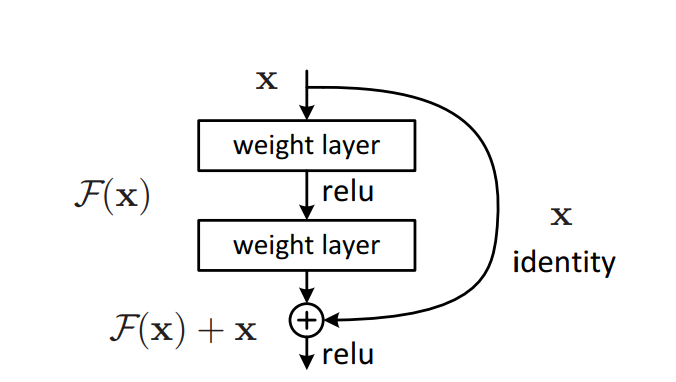
\includegraphics[width=0.6\columnwidth]{pic/resnet.png}
    \caption{ResNet网络中快捷连接示意图,可以看出输入量X被直接引入到输出中,从而使得网络$\mathcal{F}(X)$部分不会带来过多的误差。}
    \label{fig:resnet}
\end{figure}
\begin{table}
    \centering
    \begin{tabular}{ccccc}
      \\\hline
  layer name & layer type &  output tensor  & layer attribute & repetition \\\hline
  input\_1  & InputLayer & 240, 240, 3 &  & \\ \hline
  conv1 block & Convolution2D & 120, 120, 64 & 7$\times$7, 64 &  \\ \hline
  pooling & MaxPooling2D & 59, 59, 64 &  &  \\ \hline
  \multirow{3}{*}{conv2 block} & Convolution2D & 59, 59, 64 & 1$\times$1, 64 & \multirow{3}{*}3\\
   & Convolution2D & 59, 59, 64 & 3$\times$3, 64 & \\
   & Convolution2D & 59, 59, 256 & 1$\times$1, 256 & \\ \hline
  \multirow{3}{*}{conv3 block} & Convolution2D & 30, 30, 128 & 1$\times$1, 128 & \multirow{3}{*}{4} \\
   & Convolution2D & 30, 30, 128 & 3$\times$3, 128 & \\
   & Convolution2D & 30, 30, 512 & 1$\times$1, 512 & \\ \hline
  \multirow{3}{*}{conv4 block} & Convolution2D & 15, 15, 256 & 1$\times$1, 256 & \multirow{3}{*}{6} \\
   & Convolution2D & 15, 15, 256 & 3$\times$3, 256 & \\
   & Convolution2D & 15, 15, 1024 & 1$\times$1, 1024 & \\ \hline
  \multirow{3}{*}{conv5 block} &  Convolution2D & 8, 8, 512 & 1$\times$1, 512 & \multirow{3}{*}{3}\\
   & Convolution2D & 8, 8, 512 & 3$\times$3, 512 & \\
   & Convolution2D & 8, 8, 2048 & 1$\times$1, 2048 & \\ \hline
  pooling & AveragePooling2D & 1, 1, 2048 &  & \\ \hline
  flatten & Flatten & 2048 &  & \\ \hline
  dense & Dense & 256 & relu & \\  \hline
  dropout & Dropout & 256 &  & \\   \hline
  dense & Dense & 1 & sigmoid & \\ \hline
    \end{tabular}
    \caption{修改后的ResNet网络结构示意表,表中“repetition”表示网络块重复堆叠的次数,默认是1。网络中部分层以及快捷连接被省略,关于Resnet50核心部分的组成请参见论文\cite{he2016deep}。}
    \label{tab:resnet}
  \end{table}

我们使用Keras\supercite{keras}深度学习框架来构建并训练我们的CNN网络。Keras使用Python作为框架的主要语言,并可以使用由Google推出的Tensorflow\supercite{tensorflow}张量计算框架来进行具体的计算,因而可以应用由英伟达公司推出的CUDA显卡计算平台以及cuDNN\supercite{cudnn}库来加速训练的过程。训练中我们使用了一台配置了2块Nvidia Geforce 1080显卡的工作站,一共训练了30轮(epochs\footnote{一轮是指所有的训练数据通过一次神经网络。}),每轮训练后得到的权重信息都被保存了下来以供记下来的分析。在训练过程中为了降低过拟合同时搞笑的利用数据,我们对于输入图片也做了实时的数据提升,具体的训练细节见附录\ref{section:train_details}。训练操作总共耗时约5天。
  
\section{训练结果分析}
\label{section:cnn_result}

判断一个神经网络优劣的最为直观的指标之一便是准确度(accuracy),在分类模型中,它被定义为正确分类的样本数目与总样本数目的比值,用于标示该网络预测结果与真实结果的偏离程度。图\ref{fig:train_par}展示了在我们训练过程中,网络的准确度的变化趋势。
可以看出随着训练的逐步进行,训练数据集的准确度不断增加。但在20轮后训练数据集的准确度明显超过了验证数据集,即发生了过拟合现象(overfit)。因此我们选择训练集和测试集准确度比较接近但又没有发生过拟合现象的训练结果作为继续研究的对象,即第16轮到第20轮训练得到的网络权重。

\begin{figure}
    \centering
    \includegraphics[width=0.6\linewidth]{pic/04_resnet_tendency.pdf}
    \caption{训练过程中网络准确度随训练轮数的变化趋势。红色数据点表示训练集数据的准确度,蓝色数据点标示验证数据集的准确度。}
    \label{fig:train_par}
\end{figure}

在完成训练得到对应的网络权重之后,我们就可以将权重加载到我们的CNN网络模型中,并用它来预测未知的事件。因而通过上文的训练,我们得到了5组不同的网络权重,也就得到了5个CNN网络(后文称之为Model-16至Model-20)。对于任一一个输入的事件图片,它们各自都可给出一个0到1之间的数$\kappa$,表征该事件更为接近一个背景事件(0),抑或更为接近一个信号事件(1)。图\ref{fig:cnn_dis}绘制了加载第16轮训练权重的网络(Model-16),预测测试数据集所得到的$\kappa$的分布。

\begin{figure}
    \centering
    \includegraphics[width=0.6\linewidth]{pic/05_resnet_distribution.pdf}
    \caption{Model-16对于测试集数据的预测结果分布图。当$\kappa$接近1时背景事件的增多是因为的确有部分背景的径迹类似于NLDBD事件的径迹。}
    \label{fig:cnn_dis}
\end{figure}

单纯的使用准确度并不能较好的评价网络的效果,因而需要引入其他的评价方式来从上述5个网络中挑选出最好的一个。对于每个网络我们可以通过为$\kappa$设置一个阈值($\kappa_c$)来区分背景和信号,这样就可以给出每个网络的信号以及背景效率曲线。图\ref{fig:cnn_eff}上半部分给出了Model-16在不同阈值处的效率曲线。阈值的选择可以通过优化FOM(figure of merit)指标来完成,它一般被定义为最终探测到的信号的数目与背景数目开方的比值,即:
\begin{equation}
    FOM \propto \frac{s}{\sqrt{b}}=\frac{s_d}{\sqrt{b_d}}\cdot \frac{\epsilon_{s,cnn}}{\sqrt{\epsilon_{b,cnn}}}\propto \frac{\epsilon_{s,cnn}}{\sqrt{\epsilon_{b,cnn}}}
\end{equation}
其中$\epsilon_{s,cnn}$和$\epsilon_{b,cnn}$即为在选定阈值$\kappa_c$后网络的信号效率和背景效率,$s_d$和$b_b$指在未经CNN网络处理前,探测器得到的信号数目以及背景数目。

\begin{figure}
    \centering
    \includegraphics[width=0.6\linewidth]{pic/06_efficiency.pdf}
    \caption{上半部分:Model-16网络的信号效率(红线)以及背景拒绝效率(蓝线)随$\kappa_c$变化图。下半部分:效率比$\epsilon_{s,cnn}/\sqrt{\epsilon_{b,cnn}}$随$\kappa_c$变化示意图。最优$\kappa_c$位置由绿色虚线绘制出。}
    \label{fig:cnn_eff}
\end{figure}

根据PandaXIII中期报告中的计算,TPC所能探测到的NLDBD事件的半衰期与FOM成正比,因而可以通过最优化$\epsilon_{s,cnn}/\sqrt{\epsilon_{b,cnn}}$来选择网络的cut位置$\kappa_c$。图\ref{fig:cnn_eff}下半部分展示了Model-16中$\epsilon_{s,cnn}/\sqrt{\epsilon_{b,cnn}}$随$\kappa_c$的变化。当$\kappa_c$位于0.983处时,事件鉴别的FOM值最大。不同网络之间的优劣差别也可以通过对比最优FOM得到,表\ref{tab:efficiencies}描述了Model-16到Model-20,5种不同权重的网络FOM相关信息,从中可以看出Model-16能够达到最优的鉴别效果。此时信号效率为47.5\%,背景拒绝率为99.43\%,即压低本地约175倍。

\begin{table}[hbt]
    \centering
    \begin{tabular}{cccccc}
      \\\hline
      epoch & optimized $\kappa_c$ & $\epsilon_{s,cnn}$ & $ 1-\epsilon_{b,cnn}$ &$\epsilon_{s,cnn}/\sqrt{\epsilon_{b,cnn}}$ & final BI\\\hline
      16 & 0.983 & 0.475 & 0.9943 & 6.264 & $1.775\times10^{-5}$ \\
      17 & 0.976 & 0.569 & 0.9916 & 6.196 & $2.605\times10^{-5}$ \\
      18 & 0.981 & 0.487 & 0.9936 & 6.098 & $1.968\times10^{-5}$ \\
      19 & 0.966 & 0.540 & 0.9923 & 6.165 & $2.369\times10^{-5}$ \\
      20 & 0.976 & 0.520 & 0.9928 & 6.145 & $2.215\times10^{-5}$ \\\hline
      average &  &  &  & $6.174\pm0.055$ \\\hline
  %    std. err. &  & &  & 0.055 \\\hline
    \end{tabular}
    \caption{不同权重网络的最优$\kappa_c$以及对应的信号效率$\epsilon_{s,cnn}$,背景拒绝率$1-\epsilon_{b,cnn}$,$\epsilon_{s,cnn}/\sqrt{\epsilon_{b,cnn}}$和最终的本底水平(BI,单位:count$\cdot$kg$^{-1}\cdot$keV$^{-1}\cdot$year$^{-1}$)。BI计算过程中使用了 $3.088\times10^{-3}$ count$\cdot$kg$^{-1}\cdot$keV$^{-1}\cdot$year$^{-1}$ 作为未经CNN网络鉴别时的本底水平。}
    \label{tab:efficiencies}
  \end{table}
  
% vim:ts=4:sw=4
